\begin{refsection}
%************************************************
\chapter{Preliminaries}
\label{ch:preliminaries}
%************************************************

{\sffamily\slshape This chapter is identical to Appendix A and B of the published version of the preprint at \href{https://arxiv.org/abs/2504.10609}{arXiv:2504.10609}.\\}

While one might choose to represent a reaction formally by \eqref{chemical_equation}, for more practical scenarios, it is just a collection of reactant molecules (with their multiplicities) that gets converted into a collection of product molecules (with some different multiplicities). For example,\\

\begin{center}
\begin{tiny}
\begin{tabular}{ccccccc}
     \textcolor{Blue}{$e_1$} &\textcolor{Blue}{:} &\textcolor{Blue}{\chemfig{HO-[:30]-[:-30]~[:-30]N}} &\textcolor{Blue}{+} &\textcolor{Blue}{\chemfig{H_2O}} &\textcolor{Blue}{$\longrightarrow$} &\textcolor{Blue}{\chemfig{HO-[:-30]-[:30](-[:90]OH)=[:-30]NH}} \\
     && \textcolor{Blue}{$v_0$} && \textcolor{Blue}{$v_2$} && \textcolor{Blue}{$v_3$}
\end{tabular}
\vspace{0.5cm}
\end{tiny}
\end{center}

This reaction is a two-to-one map which converts molecules $\{v_0, v_1\}$ to $\{v_3\}$. In a hypergraph, we choose to represent this map graphically as
\begin{center}
    \begin{tikzpicture}[scale=1.0, color=Blue]    
        \tikzset{
        	vertex/.style = {shape=circle, line width=1pt, draw = Blue, text = Blue, align = center},
        	vertex2/.style = {shape=rectangle, line width=0.5pt, draw = Blue, text = Blue, align = center},    
            edge/.style = {->, color=Blue, line width = 2pt, -{Stealth[length=8, width=6]}}
        }        
        % vertices
        \node[vertex] (v0) at  (0,1) {$v_0$};
        \node[vertex] (v2) at  (0,0) {$v_2$};
        \node[vertex2] (e1) at  (1.2,0.5) {\tiny{$e_1$}};
        \node[vertex] (v3) at  (2.5,0.5) {$v_3$};
        \draw[edge] (v0) to (e1);
        \draw[edge] (v2) to (e1);
        \draw[edge] (e1) to (v3);
    \end{tikzpicture}
\end{center}

This object is called an hyperedge and the individual molecules $v_0$, $v_2$ and $v_3$ form the vertices. However, in a practical scenario, when the molecules $v_0$ and $v_2$ are allowed to react, reaction $e_1$ is not the only reaction that would occur and the system would not stop reacting after producing $v_3$. Successive reactions might also be possible, some of which might be:

\begin{center}
\begin{tiny}
\textcolor{Blue}{
\begin{tabular}{cccccc}
     $e_1$: &\chemfig{H_2O} + &\chemfig{HO-[:30]-[:-30]~[:-30]N} &$\rightarrow$ &\chemfig{HO-[:-30]-[:30](-[:90]OH)=[:-30]NH} \\
     & $v_2$ & $v_0$ && $v_3$ \\[4mm]
     $e_2$: &\chemfig{H_2O} + &\chemfig{HO-[:-30]-[:30](-[:90]OH)=[:-30]NH} &$\rightleftarrows$ &\chemfig{HO-[:-30]-[:30](-[:120]HO)(-[:60]OH)-[:-30]NH_2} \\
     & $v_2$ & $v_3$ && $v_4$ \\[4mm]
     $e_3$: &&\chemfig{HO-[:-30]-[:30](-[:90]OH)=[:-30]NH} &$\rightleftarrows$ &\chemfig{HO-[:-30]-[:30](=[:90]O)-[:-30]NH_2}\\
     && $v_3$ && $v_5$ \\[4mm]
     $e_4$: &\chemfig{H_2O} + &\chemfig{HO-[:-30]-[:30](=[:90]O)-[:-30]NH_2} &$\rightleftarrows$ &\chemfig{HO-[:-30]-[:30](-[:120]HO)(-[:60]OH)-[:-30]NH_2} \\
     & $v_2$ & $v_5$ && $v_4$ \\[4mm]
     $e_5$: &&\chemfig{HO-[:-30]-[:30](-[:120]HO)(-[:60]OH)-[:-30]NH_2} &$\rightarrow$ &\chemfig{HO-[:-30]-[:30](=[:90]O)-[:-30]OH} &+ \chemfig{NH_3}\\
     && $v_4$  && $v_6$ & $v_1$ \\[4mm]
     $e_6$: &&\chemfig{HO-[:-30]-[:30](-[:90]OH)=[:-30]NH} &$\rightleftarrows$ &\chemfig{HO-[:-30]=[:30](-[:90]OH)-[:-30]NH_2} \\
     && $v_3$ && $v_7$ \\[4mm]
     $e_7$: &&\chemfig{HO-[:-30]-[:30](=[:90]O)-[:-30]NH_2} &$\rightleftarrows$ &\chemfig{HO-[:-30]=[:30](-[:90]OH)-[:-30]NH_2} \\
     && $v_5$ && $v_7$ \\[4mm]
     $e_8$: &&\chemfig{HO-[:-30]=[:30](-[:90]OH)-[:-30]NH_2} &$\rightleftarrows$ &\chemfig{O=[:-30]-[:30](-[:90]OH)-[:-30]NH_2} \\
     && $v_7$ && $v_8$ \\[4mm]
     $e_9$: &&\chemfig{O=[:-30]-[:30](-[:90]OH)-[:-30]NH_2} &$\rightleftarrows$ &\chemfig{O=[:-30]-[:30]=[:-30]O} &+\chemfig{NH_3} \\
     && $v_8$ && $v_9$ & $v_1$ \\[4mm]
     $e_{10}$: &&\chemfig{O=[:-30]-[:30](-[:90]OH)-[:-30]NH_2} &$\rightleftarrows$ &\chemfig{O=[:-30]-[:30]=[:-30]NH} &+\chemfig{H_2O} \\
     && $v_8$ && $v_{10}$ & $v_2$ \\[4mm]
     $e_{11}$: &\chemfig{H_2O} + &\chemfig{O=[:-30]-[:30](-[:90]OH)-[:-30]NH_2} &$\rightleftarrows$ &\chemfig{HO-[:-30](-[:-90]OH)-[:30](-[:90]OH)-[:-30]NH_2} \\
     &$v_2$ & $v_8$ && $v_{11}$ \\[5mm]
\end{tabular}
}
\end{tiny}
\end{center}

Some of the reactions that might occur when molecules of $v_0$ and $v_2$ are allowed to react is shown. To a chemist, not all the reactions would look feasible due to reactivity constraints on the molecules, which would disallow some of the reactions. However, all these reactions might possibly occur in the system in parallel, making it an example of a concurrent system. 
\newpage

\begin{figure}[!t]
    \centering
    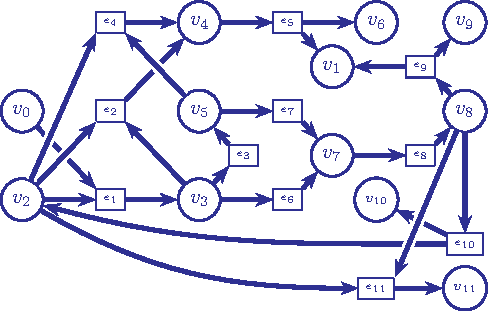
\includegraphics[scale=1.0]{graphics/chapter1/sample_network.pdf}
    \caption{A hypergraph representation of the reactions in the concurrent system.}
    \label{fig:sample_network}
\end{figure}

\begin{figure}[!h]
	\centering
	\vspace{1cm}
	\begin{subfigure}{\textwidth}
		\centering
		\begin{tiny}
		\textcolor{Blue}{
		\begin{tabular}{ccc}
			 \chemfig{HO-[:30]-[:-30]~[:-30]N} $\xrightarrow{+\chemfig{H_2O}}$ &\chemfig{HO-[:-30]-[:30](-[:90]OH)=[:-30]NH} $\xrightarrow{\text{taut.}}$ &\chemfig{HO-[:-30]=[:30](-[:90]OH)-[:-30]NH_2}\\
			 $\xrightarrow{\text{taut.}}$ \chemfig{O=[:-30]-[:30](-[:90]OH)-[:-30]NH_2} & $\xrightarrow{-\chemfig{NH_3}}$ \chemfig{O=[:-30]-[:30]=[:-30]O}
		\end{tabular}}
		\end{tiny}
		\caption{sequence of reactions forming glyoxal from glycolonitrile}
		\label{tab:sample_path1}
    \end{subfigure}
    \\
    \vspace{0.5cm}
    \begin{subfigure}{\textwidth}
    	\centering
    	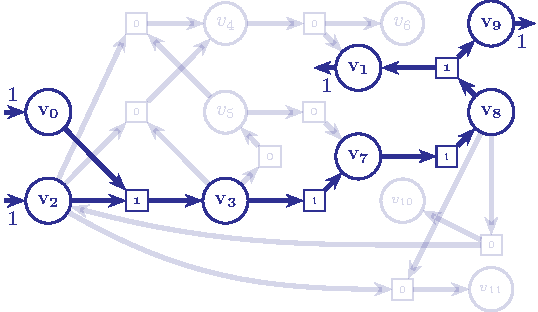
\includegraphics[scale=1.0]{graphics/chapter1/sample_path1.pdf}
    	\caption{A pathway in a hypergraph with the queried molecules $v_9$. The number in the squares denote the number of times the reaction is used to carry out the transformation or the flow assigned to the corresponding hyperedge.}
    	\label{fig:sample_path1}
	\end{subfigure}
	\vspace{0.4cm}
    \caption{The hyperflow denoting the pathway from Figure~\ref{tab:sample_path1} is shown in the hypergraph from Figure~\ref{fig:sample_network}.}
    \label{fig: samplePath1}
\end{figure}
\newpage

We would represent each reaction by a separate hyperedge and each class of molecules by a distinct vertex. This results in the structure shown in Figure~\ref{fig:sample_network}.
The reverse reactions are omitted from the hypergraph in Figure~\ref{fig:sample_network} to reduce clutter. However, in our actual modeling, we do add separate hyperedges to represent the forward and backward directions of reversible reactions.

This data structure representing the concurrent set of reactions in the system is called a multi-directed hypergraph or for simplicity, just a hypergraph. An advantage of using this data structure is that is faithfully represents the many-to-many mappings which are present in reactions which are not unimolecular. Contrast this with a simple directed graph containing edges which map one vertex to another vertex, which are often used to represent and study diverse networks in many situations. The hypergraph in Figure~\ref{fig: hypergraph} is an abstraction of another system of concurrent reactions.

One observes that glyoxal is represented as vertex $v_9$ in the hypergraph. One might query, how one inside this hypergraph can find a pathway producing glyoxal while using the input molecules $v_0$ and $v_2$. One possible transformation pathway is shown in Scheme~\ref{tab:sample_path1}.

Highlighting the hyperedges used in this transformation pathway in the hypergraph results in Figure~\ref{fig:sample_path1}. This sequence of reactions in a pathway can be found by formulating it as a flow query with molecules $v_0$ and $v_2$ as the source molecules and $v_9$ as the target molecule. The ILP assigns integers to the hyperedges which denote the number of times the hyperedge is used in the pathway. Since the flows assigned to the hyperedges are constrained to be integers, this is called an integer hyperflow. The motivation behind using allowing only non-negative integers as permissible hyperflows on a hyperedge is discussed in Section~\ref{sec: discussions}.

Often, there might exist alternative solutions to the flow query. In this case, there exists another valid integer hyperflow to the same flow query in the network with molecules $v_0$ and $v_2$ as the source molecules and $v_9$ as the target molecule which is shown in Figure~\ref{fig:sample_path2}

\begin{figure}[!t]
    \centering
    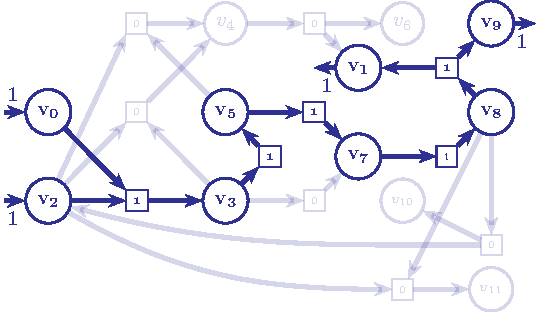
\includegraphics[scale=1.0]{graphics/chapter1/sample_path2.pdf}
    \caption{An alternative pathway to the same flow query as in Figure~\ref{fig:sample_path1}.}
    \label{fig:sample_path2}
\end{figure}

It might so happen than the reaction $v_3 \rightarrow v_7$ is slow (because it has a high energy barrier) and the two step process $v_3 \rightarrow v_5 \rightarrow v_7$ is faster. To judge which of the two pathways is better, a score is assign to them by evaluating an objective function (expression \eqref{proposed_objective} is used in this work) on the pathway, and the one with a better score is ranked higher. This automated search for pathways in a reaction system represented as a hypergraph is the motivation behind introducing the formalism of integer hyperflows in Chapter~\ref{ch:toolbox}.

\section{Generation of Reaction networks}
\label{second appendix}

There exists a diverse range of reactions. However, they are often grouped together on the basis of their mechanisms to create classes of reactions. Reactions in a class share some properties: the reactive core (type of atoms taking part in the reaction), the bonds that are broken, the movement of elections, and the new bonds that are formed. We choose to represent these classes of reactions using reaction templates. Each template defines a change in the bondset of the molecules that take part in the reaction.

For example, in the list of reaction depicted in the hypergraph~\ref{fig:sample_network}:
\begin{itemize}
    \item reactions $e_3$, $e_5$, $e_6$ $e_7$ and $e_8$ have a 1,3-shift of a hydrogen atom (often called tautomerism).
    \item reactions $e_2$, $e_4$ and $e_{11}$ are additions to an trigonal planar carbon to produce a tetrahedral carbon.
    \item reactions $e_9$ and $e_{10}$ eliminate a small molecule from a carbon with two or more adjacent electronegative atoms to form a trigonal planar carbon.
    \item reaction $e_1$ is an addition to a linear carbon to produce a trigonal carbon.
\end{itemize}
Some might prefer more fine-grained reaction templates. For instance, one might define separate templates for keto-enol tautomerism, amide-iminol tautomerism or imine-enamine tautomerism, and similarly for addition to a trigonal planar carbonyl carbon atom and addition to a trigonal planar imine carbon atom. However, that is simply a question of the level of abstraction that the user chooses to work with.

\subsection{Graph transformation rules}
We choose to represent molecules using undirected labeled graphs (hereafter called molecular graphs). The nodes in the graph represent atoms labeled by the symbol of the element, and can carry attributes such as the charge on the atom. The edges in the graph represent bonds labeled by the bond type (single, double, triple or aromatic). with this representation of molecules, the reaction templates used to abstract reactions become graph transformation rules.

A graph transformation rule consists of a subgraph on the left side which can be replaced by the subgraph on the right side when a match of the left-hand side is found in an already existing molecular graph in the network. In other words, the rule converts a part of the graph (representing a fragment of a molecule) and performs a chemical reaction. Let's consider the exchange of hydrogen atoms between oxygen atoms in a carboxylic acid.

\begin{center}
\begin{tiny}
\textcolor{Blue}{
\begin{tabular}{ccc}
     \chemfig{HO-[:30]([:90]=O)-[:-30]R} &$\rightarrow$ &\chemfig{O=[:30]([:90]-OH)-[:-30]R} 
\end{tabular}}
\end{tiny}
\end{center}

The graph transformation rule for this class of reactions would be:
\begin{center}
    \begin{tikzpicture}[scale=1.0]    
        \tikzset{
            arrow/.style = {->, -{Stealth[length = 5pt]}},
            bond/.style={line width=0.6pt},
            dbond/.style={double, double distance=2pt}
        }
        % vertices
        \node (c0) at (0,0) {C};
        \node (o1) at (1,0) {\textcolor{red}{O}};
        \node (o2) at (0,-1) {\textcolor{red}{O}};
        \node (h3) at (1,-1) {H};
        \draw[bond] (c0) to (o2);
        \draw[bond] (o2) to (h3);
        \draw[dbond] (c0) to (o1);

        \draw[arrow] (2,-0.5) to (3,-0.5);

        \node (c0) at (4,0) {C};
        \node (o1) at (5,0) {\textcolor{red}{O}};
        \node (o2) at (4,-1) {\textcolor{red}{O}};
        \node (h3) at (5,-1) {H};
        \draw[dbond] (c0) to (o2);
        \draw[bond] (o1) to (h3);
        \draw[bond] (c0) to (o1);
    \end{tikzpicture}
\end{center}

The amide-iminol conversion is a more substantial example.
\begin{center}
\begin{tiny}
\textcolor{Blue}{
\begin{tabular}{ccc}
     \chemfig{H_2N-[:30]([:90]=O)-[:-30]R} &$\rightarrow$ &\chemfig{HN=[:30]([:90]-OH)-[:-30]R} 
\end{tabular}}
\end{tiny}
\end{center}

The graph transformation rule for this class of reactions would be:
\begin{center}
    \begin{tikzpicture}[scale=1.0]    
        \tikzset{
            arrow/.style = {->, -{Stealth[length = 5pt]}},
            bond/.style={line width=0.6pt},
            dbond/.style={double, double distance=2pt}
        }
        % vertices
        \node (c0) at (0,0) {C};
        \node (o1) at (1,0) {\textcolor{red}{O}};
        \node (n2) at (0,-1) {\textcolor{blue}{N}};
        \node (h3) at (1,-1) {H};
        \draw[bond] (c0) to (n2);
        \draw[bond] (n2) to (h3);
        \draw[dbond] (c0) to (o1);

        \draw[arrow] (2,-0.5) to (3,-0.5);

        \node (c0) at (4,0) {C};
        \node (o1) at (5,0) {\textcolor{red}{O}};
        \node (n2) at (4,-1) {\textcolor{blue}{N}};
        \node (h3) at (5,-1) {H};
        \draw[dbond] (c0) to (n2);
        \draw[bond] (o1) to (h3);
        \draw[bond] (c0) to (o1);
    \end{tikzpicture}
\end{center}
This rule rewrites an amide fragment when it is found in a molecule with an iminol fragment, thus effecting the required reaction.

For a keto-enol tautomerism like
\begin{center}
\begin{tiny}
\textcolor{Blue}{
\begin{tabular}{ccc}
     \chemfig{R'-[:-30](-[:-90]H)-[:30]([:90]=O)-[:-30]R} &$\rightarrow$ &\chemfig{R'-[:-30]=[:30]([:90]-OH)-[:-30]R} 
\end{tabular}}
\end{tiny}
\end{center}

the graph transformation rule for this class of reactions would be:
\begin{center}
    \begin{tikzpicture}[scale=1.0]    
        \tikzset{
            arrow/.style = {->, -{Stealth[length = 5pt]}},
            bond/.style={line width=0.6pt},
            dbond/.style={double, double distance=2pt}
        }
        % vertices
        \node (c0) at (0,0) {C$^1$};
        \node (o1) at (1,0) {\textcolor{red}{O}};
        \node (c2) at (0,-1) {C$^2$};
        \node (h3) at (1,-1) {H};
        \draw[bond] (c0) to (c2);
        \draw[bond] (c2) to (h3);
        \draw[dbond] (c0) to (o1);

        \draw[arrow] (2,-0.5) to (3,-0.5);

        \node (c0) at (4,0) {C$^1$};
        \node (o1) at (5,0) {\textcolor{red}{O}};
        \node (c2) at (4,-1) {C$^2$};
        \node (h3) at (5,-1) {H};
        \draw[dbond] (c0) to (c2);
        \draw[bond] (o1) to (h3);
        \draw[bond] (c0) to (o1);
    \end{tikzpicture}
\end{center}
Note that the graph transformation rule indicates the bare minimum that is required to be present as a subgraph in the molecule for the reaction to occur. For example, the carbon at the 2-position, might have two adjacent hydrogen atoms, but the rule specifies that at least one hydrogen atom is required for the keto isomer to convert into the enol isomer. Without any hydrogen at the 2-position, the fragment on the left is not a subgraph of the molecule and this transformation rule cannot be applied to the graph.

Also, note that the objective here is not to capture the exact mechanism of the reaction, but rather specify what the molecular fragment is before and after the reaction. In all the three reactions mentioned above, the 1,3-hydrogen transfer involves a solvent molecule. In most cases, it is not the exact same hydrogen atom that would be in the molecule before and after the reaction.

The similarity in the graph transformation rule for the three reactions mentioned above above look similar. For a more elegant formulation, we define the following graph transformation rule to account for all the three cases above:
\begin{center}
    \begin{tikzpicture}[scale=1.0]    
        \tikzset{
            arrow/.style = {->, -{Stealth[length = 5pt]}},
            bond/.style={line width=0.6pt},
            dbond/.style={double, double distance=2pt}
        }
        % vertices
        \node (c0) at (0,0) {C};
        \node (o1) at (1,0) {$\mathcal{Y}$};
        \node (c2) at (0,-1) {$\mathcal{X}$};
        \node (h3) at (1,-1) {H};
        \draw[bond] (c0) to (c2);
        \draw[bond] (c2) to (h3);
        \draw[dbond] (c0) to (o1);

        \draw[arrow] (2,-0.5) to (3,-0.5);

        \node (c0) at (4,0) {C};
        \node (o1) at (5,0) {$\mathcal{Y}$};
        \node (c2) at (4,-1) {$\mathcal{X}$};
        \node (h3) at (5,-1) {H};
        \draw[dbond] (c0) to (c2);
        \draw[bond] (o1) to (h3);
        \draw[bond] (c0) to (o1);

        \node at (2.5,-2) {$\mathcal{X}, \mathcal{Y} \in \{\text{C, N, O}\}$};
    \end{tikzpicture}
\end{center}

This graph transformation rule also encodes an allyl hydrogen shift, an imine-enamine tautomerism, or the hydrogen exchange in amidine.
\begin{center}
\begin{tiny}
\textcolor{Blue}{
\begin{tabular}{ccc}
    \chemfig{R_4-[:-30](-[:120]R_5)(-[:-90]H)-[:30]([:90]-R_3)=[:-30](-[:-90]R_2)-[:30]R_1} &$\rightarrow$ &\chemfig{R_4-[:-30](-[:-90]R_5)=[:30]([:90]-R_3)-[:-30](-[:-90]R_2)(-[:60]H)-[:30]R_1} \\\\
    \chemfig{R'-[:-30](-[:-90]H)-[:30]([:90]=NH)-[:-30]R} &$\rightarrow$ &\chemfig{R'-[:-30]=[:30]([:90]-NH_2)-[:-30]R} \\\\
    \chemfig{H_2N-[:30]([:90]=NH)-[:-30]R} &$\rightarrow$ &\chemfig{HN=[:30]([:90]-NH_2)-[:-30]R} 
\end{tabular}}
\end{tiny}
\end{center}

However, all these six different reactions are expected to have differing mechanisms. This graph transformation rule introduces two variables $\mathcal{X}, \mathcal{Y}$ which can be matched with the label C, N or O, or in other words the atoms in the place of  $\mathcal{X}, \mathcal{Y}$ in the molecular fragment can be a carbon, nitrogen or oxygen atom.

Similarly the graph transformation rule
\begin{center}
    \begin{tikzpicture}[scale=1.0]    
        \tikzset{
            arrow/.style = {->, -{Stealth[length = 5pt]}},
            bond/.style={line width=0.6pt},
            dbond/.style={double, double distance=2pt}
        }
        % vertices
        \node (c0) at (0,-1) {C};
        \node (o1) at (0,0) {$\mathcal{Y}$};
        \node (c2) at (1,-1) {$\mathcal{X}$};
        \node (h3) at (1,0) {H};
        \draw[bond] (c2) to (h3);
        \draw[dbond] (c0) to (o1);

        \draw[arrow] (2,-0.5) to (3,-0.5);

        \node (c0) at (4,-1) {C};
        \node (o1) at (4,0) {$\mathcal{Y}$};
        \node (c2) at (5,-1) {$\mathcal{X}$};
        \node (h3) at (5,0) {H};
        \draw[dbond] (c0) to (c2);
        \draw[bond] (o1) to (h3);
        \draw[bond] (c0) to (o1);

        \node at (2.5,-2) {$\mathcal{X}, \mathcal{Y} \in \{\text{N, O}\}$};
    \end{tikzpicture}
\end{center}

encodes the addition of a water or ammonia molecule to a carbonyl or imine group.
\begin{center}
\begin{tiny}
\textcolor{Blue}{
\begin{tabular}{ccc}
    \chemfig{R'-[:30]([:90]=NH)-[:-30]R} &$\xrightarrow{+\chemfig{NH_3}}$ &\chemfig{R'-[:30]([:90]-NH_2)(-[:-60]NH_2)-[:-30]R} \\\\
    \chemfig{R'-[:30]([:90]=NH)-[:-30]R} &$\xrightarrow{+\chemfig{H_2O}}$ &\chemfig{R'-[:30]([:90]-NH_2)(-[:-60]OH)-[:-30]R} \\\\
    \chemfig{R'-[:30]([:90]=O)-[:-30]R} &$\xrightarrow{+\chemfig{NH_3}}$ &\chemfig{R'-[:30]([:90]-OH)(-[:-60]NH_2)-[:-30]R} \\\\
     \chemfig{R'-[:30]([:90]=O)-[:-30]R} &$\xrightarrow{+\chemfig{H_2O}}$ &\chemfig{R'-[:30]([:90]-OH)(-[:-60]OH)-[:-30]R} 
\end{tabular}}
\end{tiny}
\end{center}
We admit that these reactions are not a simple one step process as the transformation rule make them appear to be and not all of these possible reactions is always feasible for all reactant molecules.

In all the graph transformation rules in this section, the context graph $K$, which comes between the left and right-hand sides, is omitted. The context graph must be added to the graph transformation rules for mathematical correctness. It ensures that logically the bonds are first removed, and then added, making the graph rewriting a two-step process.

\subsection{Rule application to a graph}

When a graph transformation rule is applied to a set of reactant molecules, a reaction might occur. First, it is checked if the left-hand side of the rule, $L$, is present as a subgraph in the set of reactant molecules $G$. If so, then that subgraph is rewritten according to the rule to R, to generate a new set of molecules $H$, the product molecules. This process is illustrated in Figure~\ref{fig:rule_application1}.

\begin{figure}[!t]
    \centering
    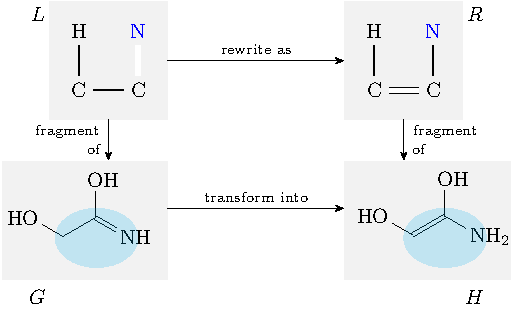
\includegraphics[width=\linewidth]{graphics/chapter1/rule_app1.pdf}
    \begin{tikzpicture}
        \draw (0, 0) -- (4, 0);
    \end{tikzpicture}
    \vspace{1.0cm}\\
    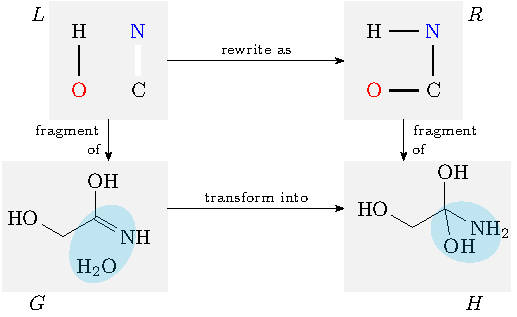
\includegraphics[width=\linewidth]{graphics/chapter1/rule_app2.pdf}
    \caption{Two examples of the application of a graph transformation rule to a collection of molecules.}
    \label{fig:rule_application1}
\end{figure}

If the left-hand side of the rule, $L$, is not present in the set of molecules $G$, then that reaction template cannot be applied to the given set of molecules.

\begin{figure}[h]
    \centering
    \begin{tikzpicture}[scale=1.0]    
        \tikzset{
            arrow/.style = {->, -{Stealth[length = 5pt]}},
            bond/.style={line width=0.6pt},
            dbond/.style={double, double distance=2pt},
            tbond/.style={double, double distance=4pt}
        }
        % vertices
        \draw[fill=gray, fill opacity=0.1, draw=none] (-0.5,-0.5) rectangle (1.5,1.5);
        \node at (-0.7, 1.3) {$L$};
        \node (c0) at (1,0) {C};
        \node (n1) at (1,1) {\textcolor{blue}{N}};
        \node (c2) at (0,0) {O};
        \node (h3) at (0,1) {H};
        \draw[bond] (c2) to (h3);
        \draw[tbond] (c0) to (n1);
        \draw[bond] (c0) to (n1);
        
        \draw[arrow] (1.5,0.5) to (4.5,0.5);
        \node at (3,0.7) {\scriptsize{rewrite as}};

        \draw[fill=gray, fill opacity=0.1, draw=none] (4.5,-0.5) rectangle (6.5,1.5);
        \node at (6.7, 1.3) {$R$};
        \node (c0) at (6,0) {C};
        \node (n1) at (6,1) {\textcolor{blue}{N}};
        \node (c2) at (5,0) {O};
        \node (h3) at (5,1) {H};
        \draw[bond] (c2) to (h3);
        \draw[bond] (c0) to (c2);
        \draw[dbond] (c0) to (n1);

        \draw[fill=gray, fill opacity=0.1, draw=none] (-1.4,-3.5) rectangle (2.2,-1.2);
        \node (lhs) at (0.5, -2.25) {\chemfig{HO-[:-30]-[:30](-[:90]OH)=[:-30]NH}};
        \node at (-1.7,-2.5) {$G$};
        
        \draw[arrow, color=red] (0.5,-0.5) to (0.5,-1.2);
        \node at (0.25,-0.7) {\scriptsize{\textcolor{red}{no}}};
        \node at (0.1,-1) {\scriptsize{\textcolor{red}{match}}};
    \end{tikzpicture}
    \caption{A case where the graph transformation rule cannot be applied to a molecule}
    \label{fig:rule_application2}
\end{figure}
Therefore, the application of a rule to an existing set of molecules might produce new molecules, which in turn expands the molecular space. Repeated application of these rules constructs a network, which is detailed in the next section.

\subsection{Construction of the reaction network}

The construction of the reaction network requires a set of input molecules and some graph transformation rules. A match between a collection of molecules and the subgraph on the left-hand side of one of the transformation rules means that this reaction template can be applied to that collection of molecules created from the input set of molecules. Thus, when a rule is applied to a collection of molecules from the current set of molecules, new molecules are created. In a generative process, these new molecules are then added to the set of available molecules (i.e., this set is updated). Graph transformation rules can be recursively applied to this new set of molecules, effecting more reactions to be made and thus the molecular space expands. The hypergraph representation of the network keeps track of all the reactions performed and of the molecules current present in the network.

\begin{figure}
    \centering
    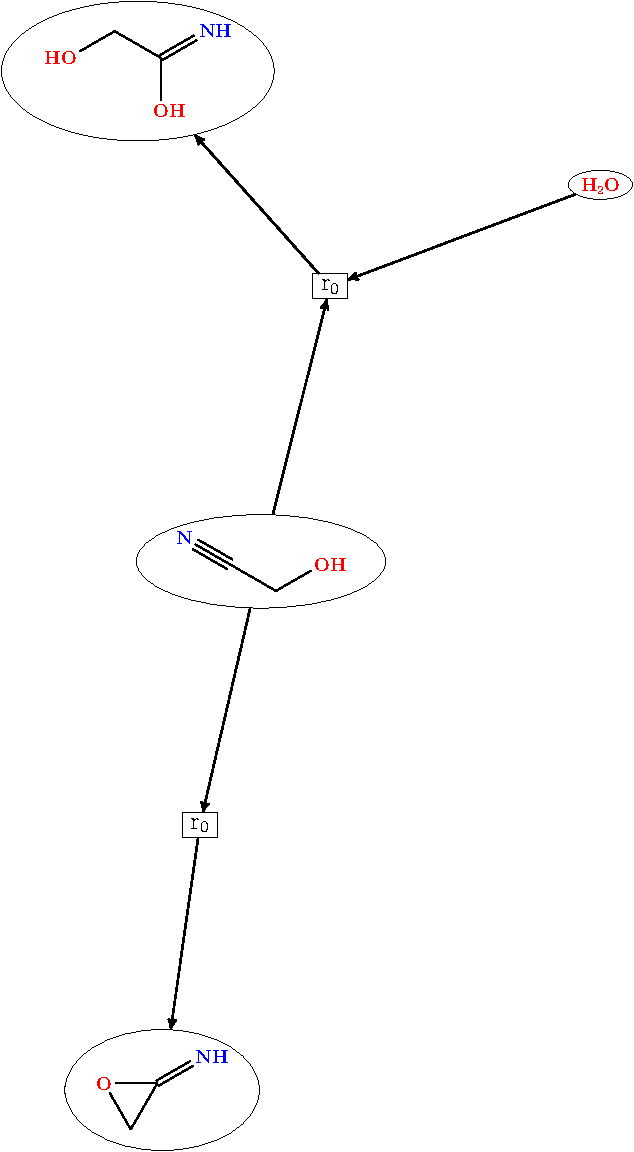
\includegraphics[scale=0.3]{graphics/chapter1/recurse1.pdf}\\
    \vspace{0.4cm}
    \begin{tikzpicture}
        \draw (0, 0) -- (4, 0);
    \end{tikzpicture}\\
    \vspace{1.0cm}
    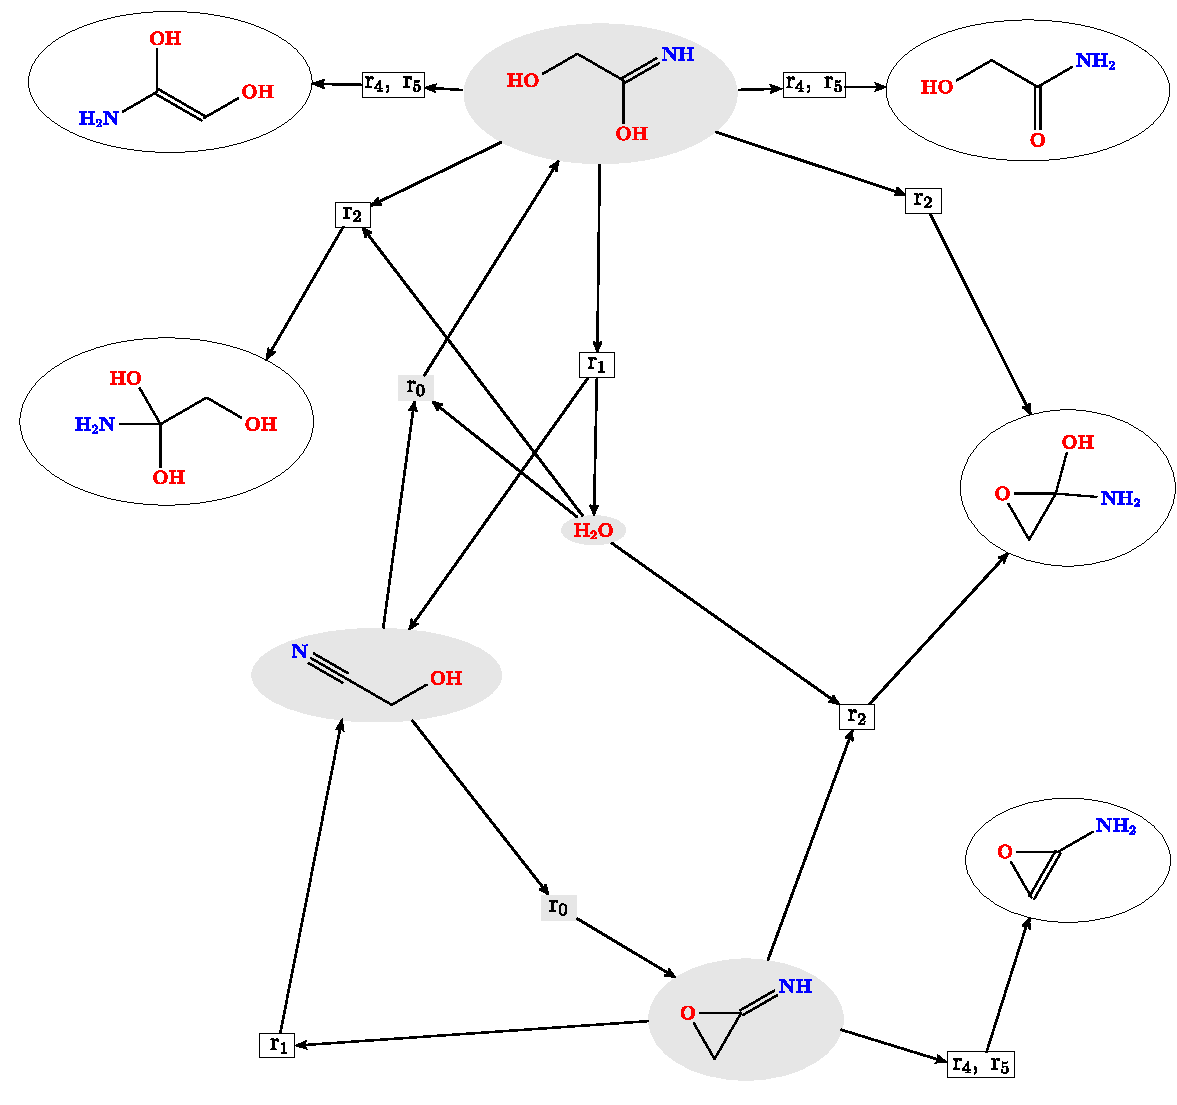
\includegraphics[scale=0.4]{graphics/chapter1/recurse2.pdf}
    \vspace{0.5cm}
    \caption{(top) The reaction network (with $4$ molecules and $2$ reactions) after one recursive application of the graph transformation rules, and (bottom) the reaction network (with $9$ molecules and $10$ reactions) after two recursive applications of the graph transformation rules. The part of the network already generated previously has been shaded.}
    \label{fig: grow_network}
\end{figure}

\begin{figure}
    \centering
    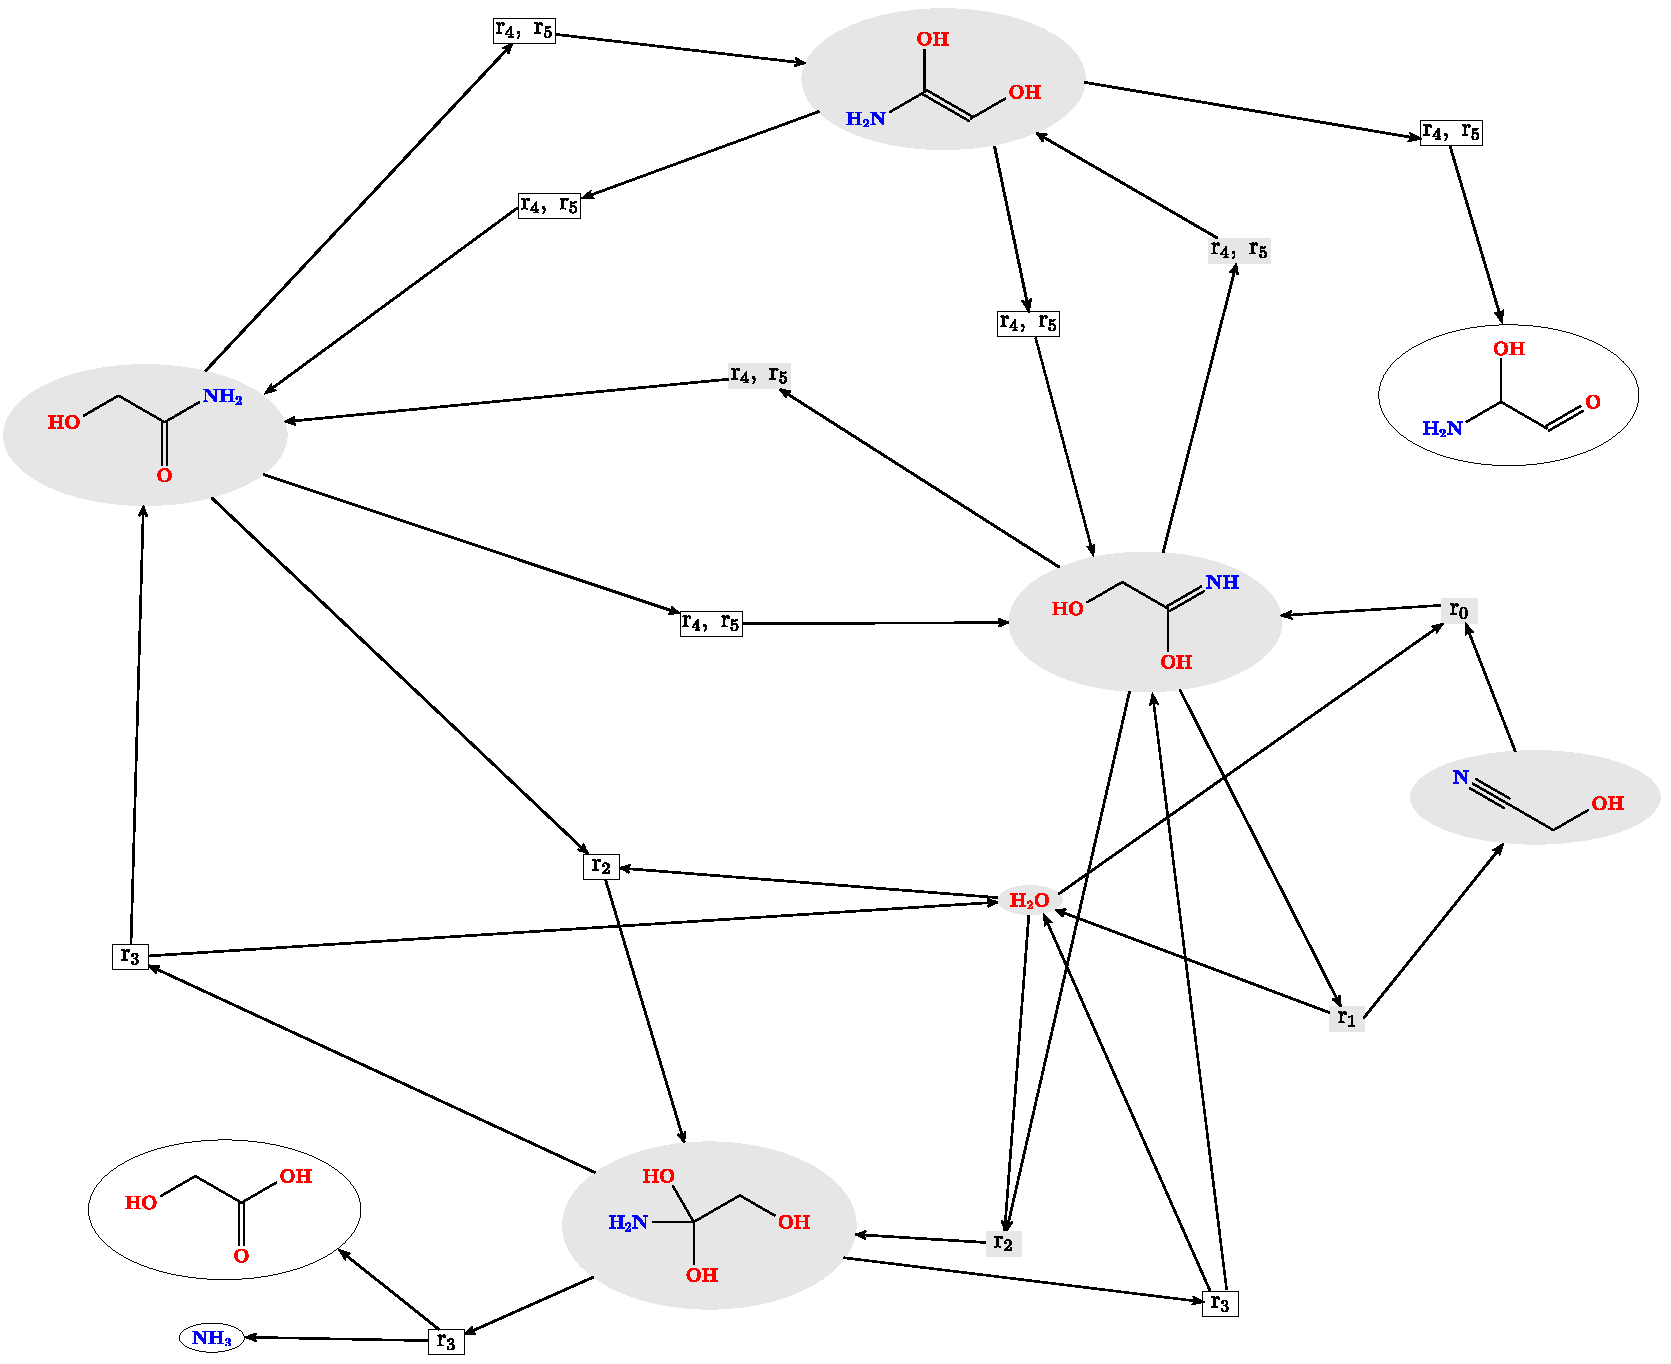
\includegraphics[width=\linewidth]{graphics/chapter1/recurse3.pdf}
    \vspace{0.5cm}
    \caption{The reaction network (with $9$ molecules and $14$ reactions) after three recursive applications of the graph transformation rules with the 3-cycles filtered out. The part of the network already generated previously has been shaded.}
    \label{fig: recurse3}
\end{figure}

To illustrate the construction of a reaction network by the recursive application of graph transformation rules to an input set of molecules, the graph transformation rules from Figure~\ref{fig:graphTransformationRules} in Chpater~\ref{ch:casestudy2} is applied to the input molecules water and 2-hydroxyethanenitrile is shown in Figures~\ref{fig: grow_network}, \ref{fig: recurse3} and \ref{fig: recurse4}.

Notice that some molecules in Figure~\ref{fig: grow_network}, such as the 3-cycles, are not realistic. One can disallow their addition to the generated reaction network by using so-called right predicates. Right predicates filter out certain reactions from the network based on the properties of the molecular graphs that appear on the right-hand side of a derivation. This, it prunes the generated network and makes its growth more manageable and potentially more realistic. The effect of using the right predicate can be seen in the hypergraph in Figure~\ref{fig: recurse3}, which has $9$ molecules after three recursive expansion steps, while the hypergraph in Figure~\ref{fig: grow_network} already had $9$ molecules after two recursive steps when the right predicate was not used.

\begin{figure}
    \centering
    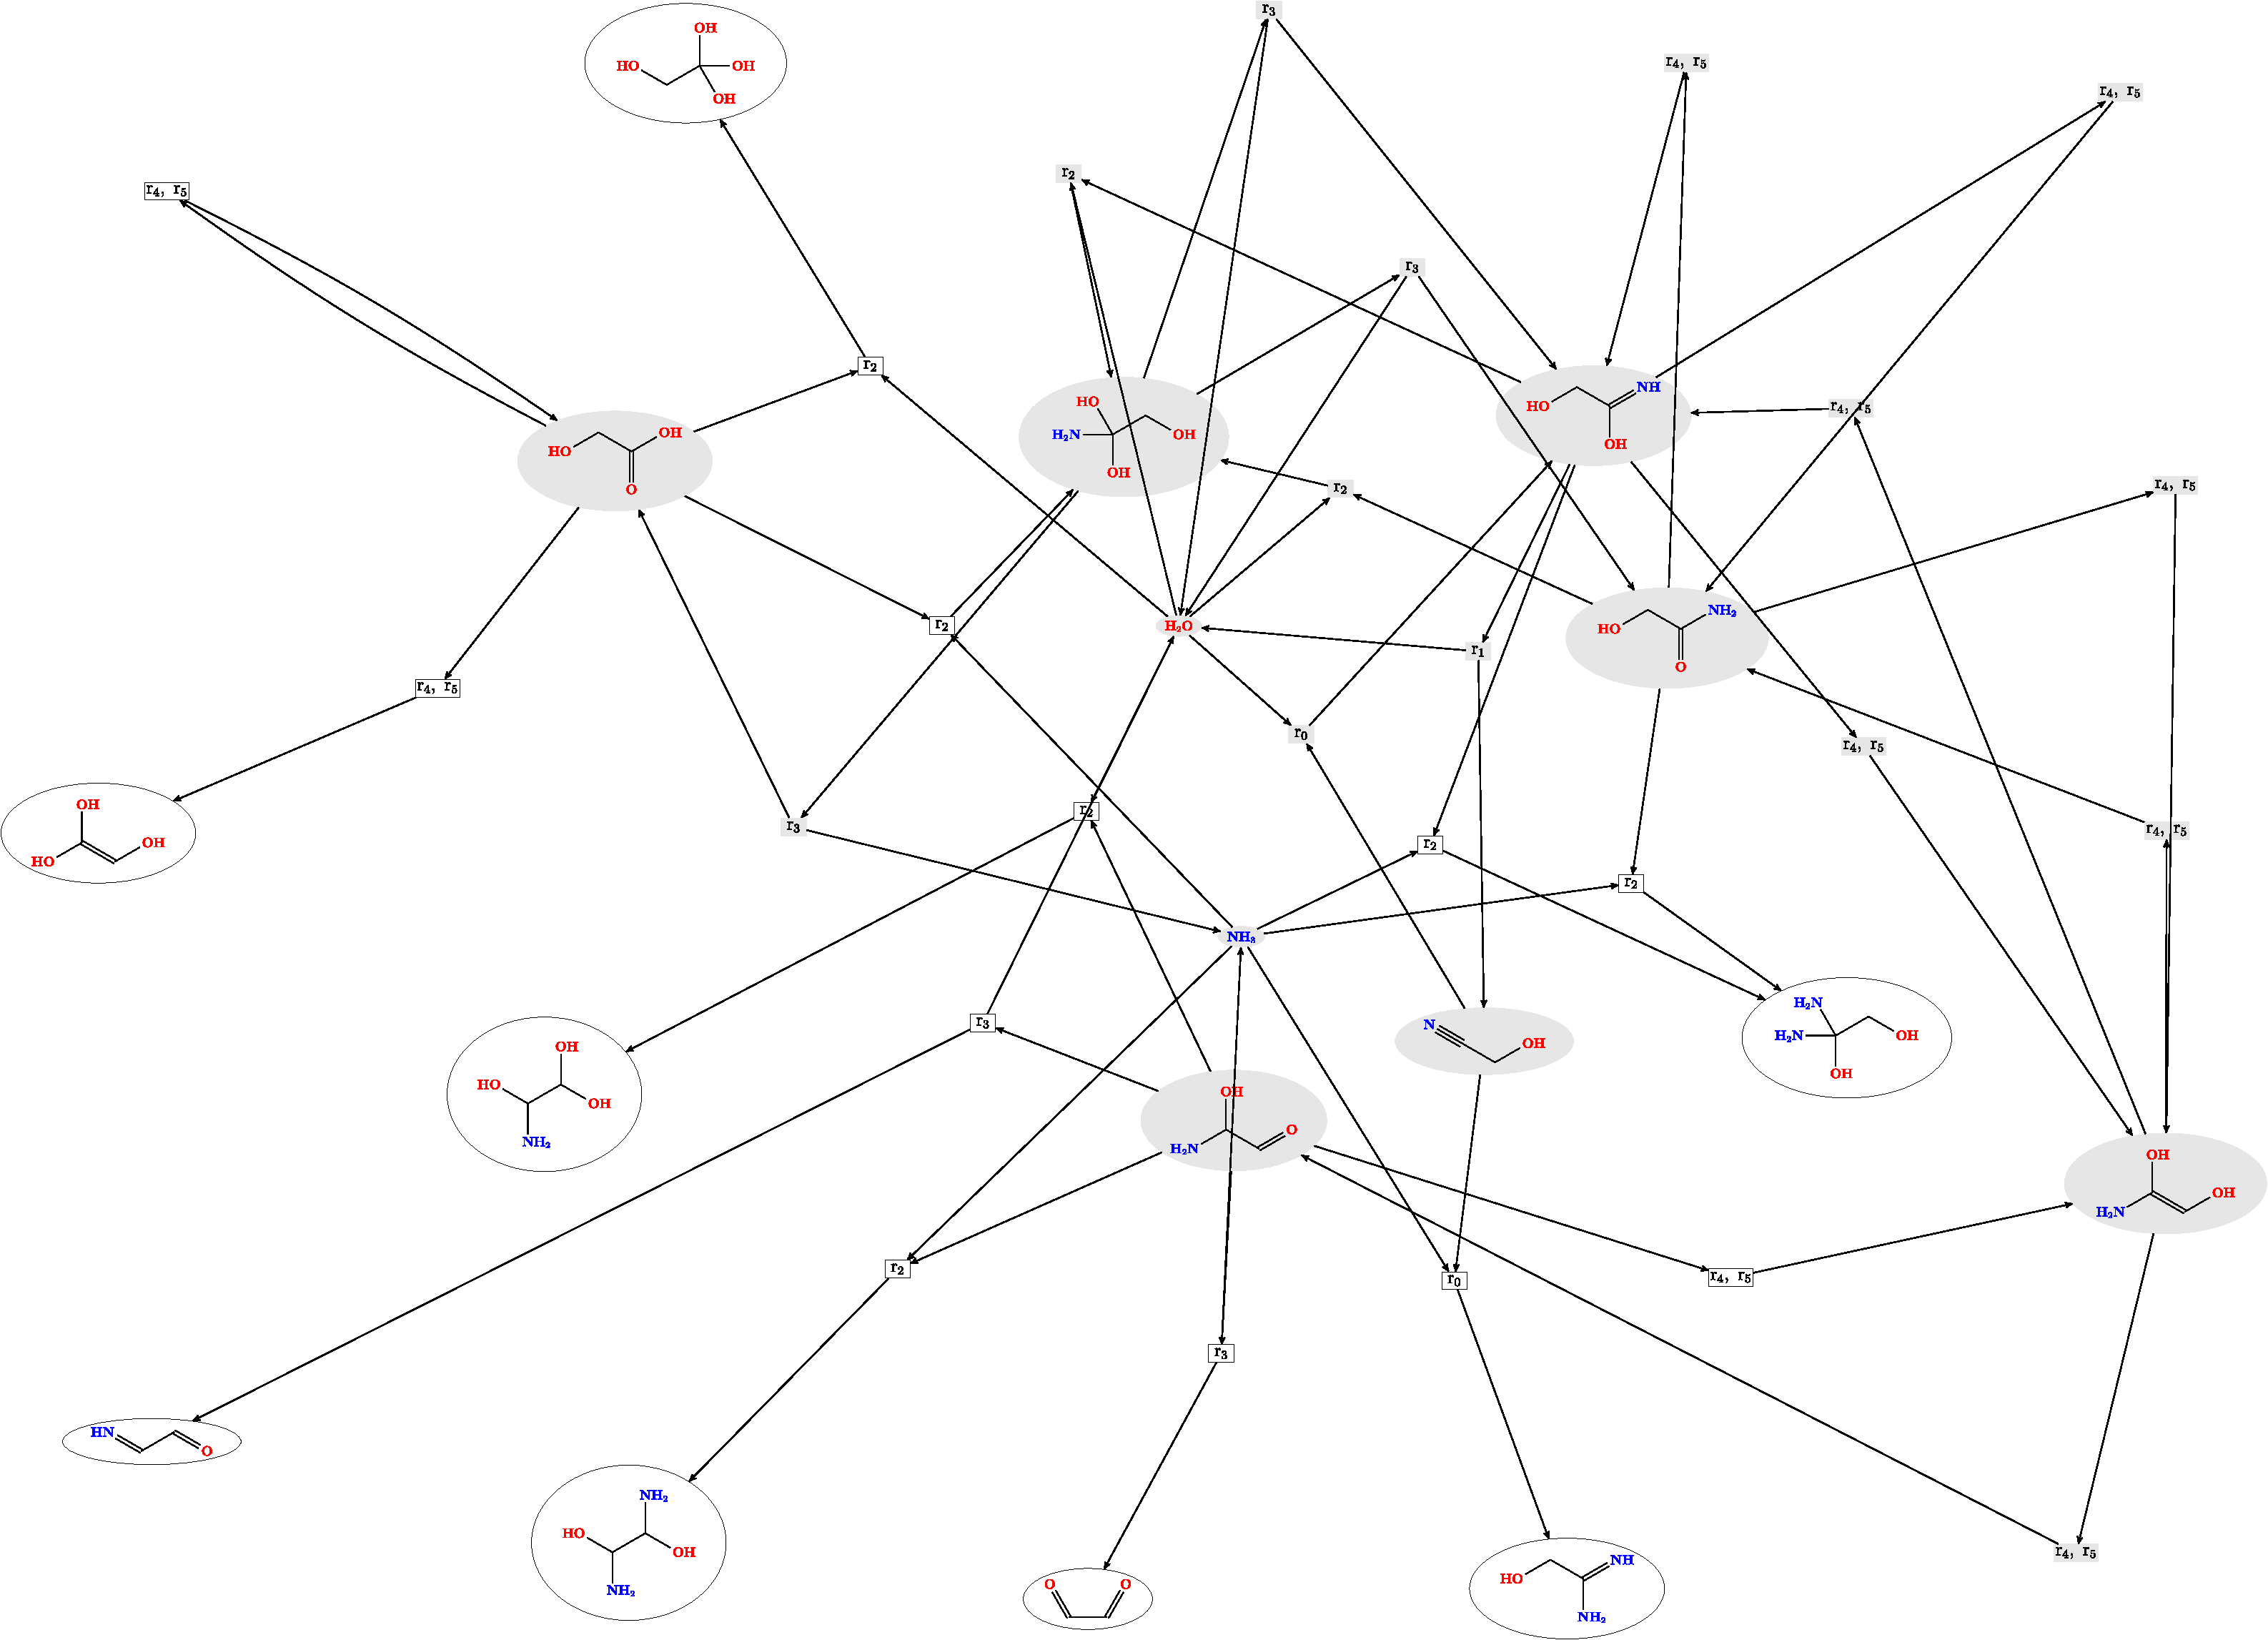
\includegraphics[width=\linewidth]{graphics/chapter1/recurse4.pdf}
    \vspace{0.5cm}
    \caption{The reaction network (with $17$ molecules and $26$ reactions) after four recursive applications of the graph transformation rules with the 3-cycles filtered out. The part of the network that was already generated aftre three recersive steps has been shaded.}
    \label{fig: recurse4}
\end{figure}

Often, one direction of a reaction is added to the hypergraph (adding new molecules to the existing set of molecules) and the reverse direction is added in the next recursion. This adds a new reaction between reactants and products both of which are already present in the set of existing molecules.
The graph transformation rules can be applied for a specified number of iterations, or until a specified limit on the size of the different molecules generated is reached which terminated the network generation process. This makes the derived hypergraph finite.

\section{Hyperflows and Fluxes}
\label{sec: comparison}

In this section, we give a comparison of our workflow with existing methods. Constraint-based models such as flux balance analysis also use constraint programming with an objective function that is optimized. For instance, open-source tools such as COBRApy~\cite{cobrapy} perform flux analysis on a reaction network supplied to them. However, such tools do not construct the network on the fly in a generative way--- rather the reaction network has to be constructed beforehand using some other tool. Flux balance analysis generates a flux vector for the reactions in the network which is allowed to contain floating-point values, while our method accepts only integers as a valid hyperflow for a reaction, which is more aligned with the standard notion of a pathway. Formulating a flux balance analysis on the network would be equivalent to an LP relaxation of the pathway query problem using integer hyperflows for the same network. A linear program (LP) can be solved in polynomial time while an ILP is NP-hard. However, formulating the search for pathways to a queried molecule in a reaction network offers some advantages.

\begin{figure}
    \centering
    \begin{subfigure}{\textwidth}
        \centering
        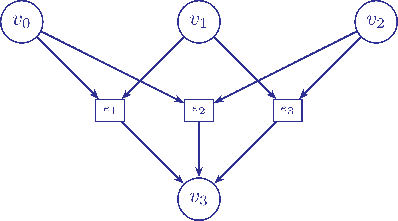
\includegraphics[scale=1.0]{graphics/chapter1/example_network.pdf}
        \vspace{0.4cm}
        \caption{An example reaction network with $4$ molecules and $3$ reactions.}
        \label{fig:example_network}
    \end{subfigure}\\
    \vspace{0.8cm}
    \begin{subfigure}{\textwidth}
        \centering
        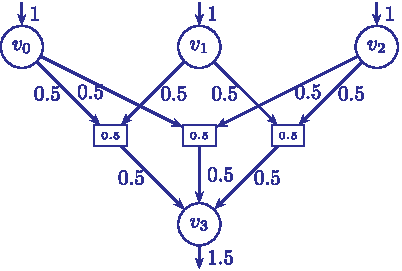
\includegraphics[scale=1.0]{graphics/chapter1/example_flux.pdf}
        \vspace{0.4cm}
        \caption{A flux distribution in the network which produces an outflow of $1.5$ for $v_3$.}
        \label{fig:example_flux}
    \end{subfigure}\\
    \vspace{0.8cm}
    \begin{subfigure}{\textwidth}
        \centering
        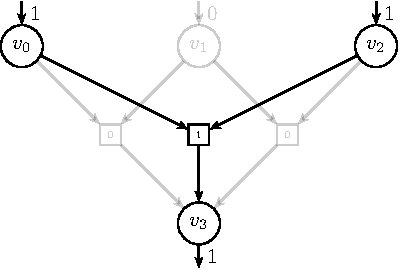
\includegraphics[scale=1.0]{graphics/chapter1/example_flow.pdf}
        \vspace{0.4cm}
        \caption{An assignment of integer hyperflows in the network which produces an outflow of $1$ for $v_3$.}
        \label{fig:example_flow}
    \end{subfigure}
    \vspace{1cm}
    \caption{Comparison of flux balance analysis and an integer hyperflow in an example reaction network.}
    \label{fig:comparison}
\end{figure}

There exists reaction networks where the optimal solutions from the ILP formulated by our modeling and the relaxed LP from flux balance analysis differ. Consider the reaction network shown in Figure~\ref{fig:example_network} with the following formulation of the problem:
\begin{align*}
    &\max \left( \text{outflow}(v_3) \right) \\
    \text{subject to: } &\text{inflow}(v_0) + \text{inflow}(v_1) +\text{inflow}(v_2) \leq 3
\end{align*}
The optimal flux distribution yields an objective value of $1.5$ with the assigned fluxes shown in Figure~\ref{fig:example_flux} while our method assigns the integer hyperflows shown in Figure~\ref{fig:example_flow} in one of the three optimal solutions with objective value $1$. The other two solutions assign the hyperflows $(0,1,1)$ and $(1,1,0)$ to the hyperedge set $(e_1,e_2,e_3)$ respectively.

The ILP solution space is a subset of the LP feasible reaction and therefore, the objective value for the optimal solution for the relaxed LP will always be as at least as large as the objective value of optimal solution for the corresponding ILP. This is illustrated in the example shown in Figure~\ref{fig:comparison} too. As the result, the fluxes and the structure of the solution is often different from those if they were constrained to be integers.

Restricting hyperflows to integers makes physical sense because molecules occur and react in discrete quantities.
Actually, small molecular counts in several biological settings (often involving trace amounts of enzymes and inhibitors affecting multiple iterations of the same pathway) and physical cases (as in chain reactions and cascades) do not allow arbitrary scaling of the number of molecules, as the use of real-valued fluxes by flux balance analysis assume.
When a small number of molecules are encountered in a scenario as above (or in scenarios with appearances of a rare but significant molecule in the system), the discrete nature of the molecules becomes more pronounced.

Another feature of our proposed method is the enumeration of alternative pathways with disjoint set of hyperedges ranked on the basis of a chosen objective function. While flux balance analysis offers the possibility to find alternative pathways~\cite{fba_alternative_pathways}, they have the same objective value but a different flux distribution in the network. This differs from the enumeration of solutions in the current method which offers a list of pathways ordered by the increasing value of the objective function for the user to choose from. Enumerating solutions over variables with a continuous domain is difficult using indicator variables and biimplications as in constraints \ref{biimp1}  and \ref{biimp2}. The enumeration of solutions offers diverse pathways to the queried molecules and makes the method more robust to uncertainties in the weights assigned to the hyperedges.

\printbibliography[
  heading=subbibliography,
  title={References}
]

\end{refsection}
